\chapter{Programación lineal}

\section{Objetivo de la programación lineal e interpretación en $\IR^3$}
El objetivo de la programación lineal es resolver el problema de
minimizar o maximizar una función $f:\IR^n\rightarrow\IR$
restringida a un dominio $D\subset\IR^n$ de manera que tanto $f$ como
$D$ cumplan ciertas condiciones.

\ifthenelse{\equal{\PDFMODE}{1}}{
  \begin{figure}[h]
    \centering
    \begin{subfigure}[b]{0.3\textwidth}
      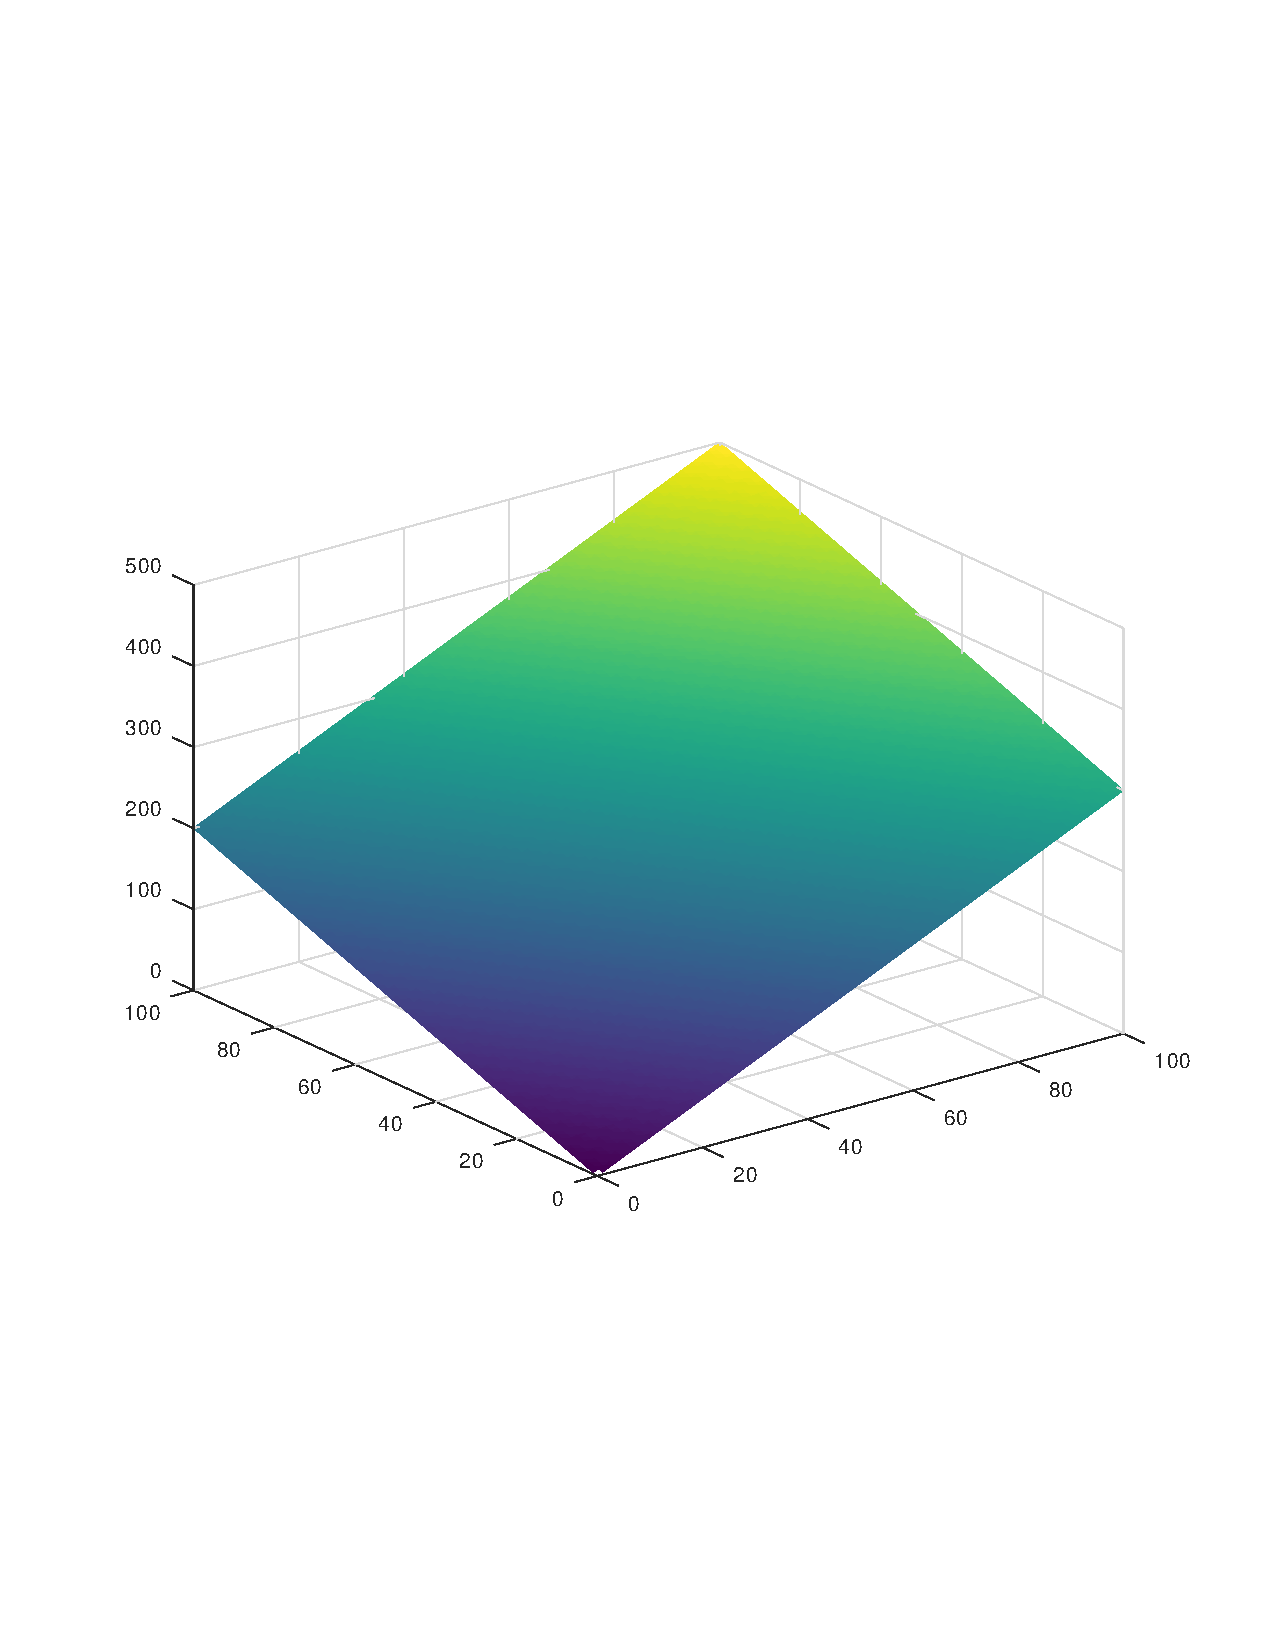
\includegraphics[width=\textwidth]{2_INTRO_1}
      \caption{Una aplicación $f$ lineal}
    \end{subfigure}
    ~ %add desired spacing between images, e. g. ~, \quad, \qquad, \hfill etc. 
    % (or a blank line to force the subfigure onto a new line)
    \begin{subfigure}[b]{0.3\textwidth}
      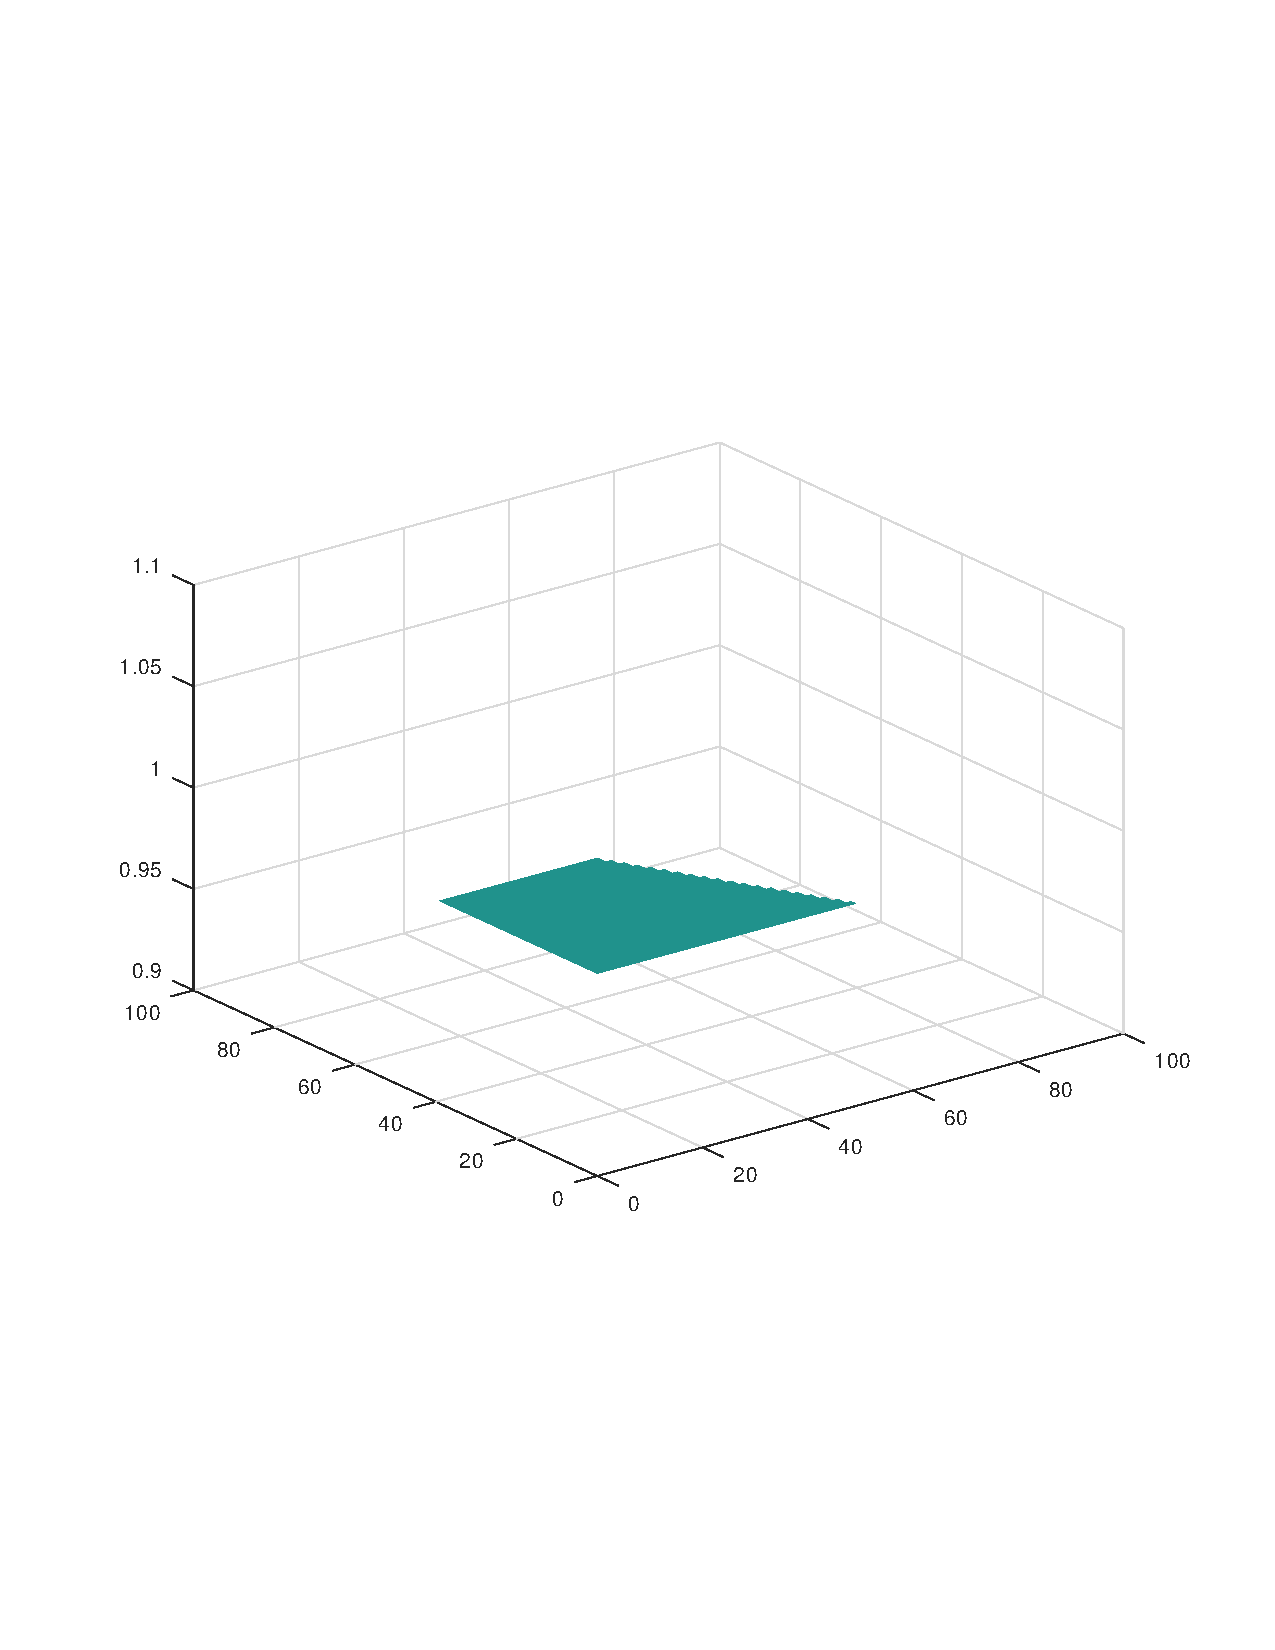
\includegraphics[width=\textwidth]{2_INTRO_2}
      \caption{Una $\mathcal{R}$ región dada por restricciones}
    \end{subfigure}
    ~ %add desired spacing between images, e. g. ~, \quad, \qquad, \hfill etc. 
    % (or a blank line to force the subfigure onto a new line)
    \begin{subfigure}[b]{0.3\textwidth}
      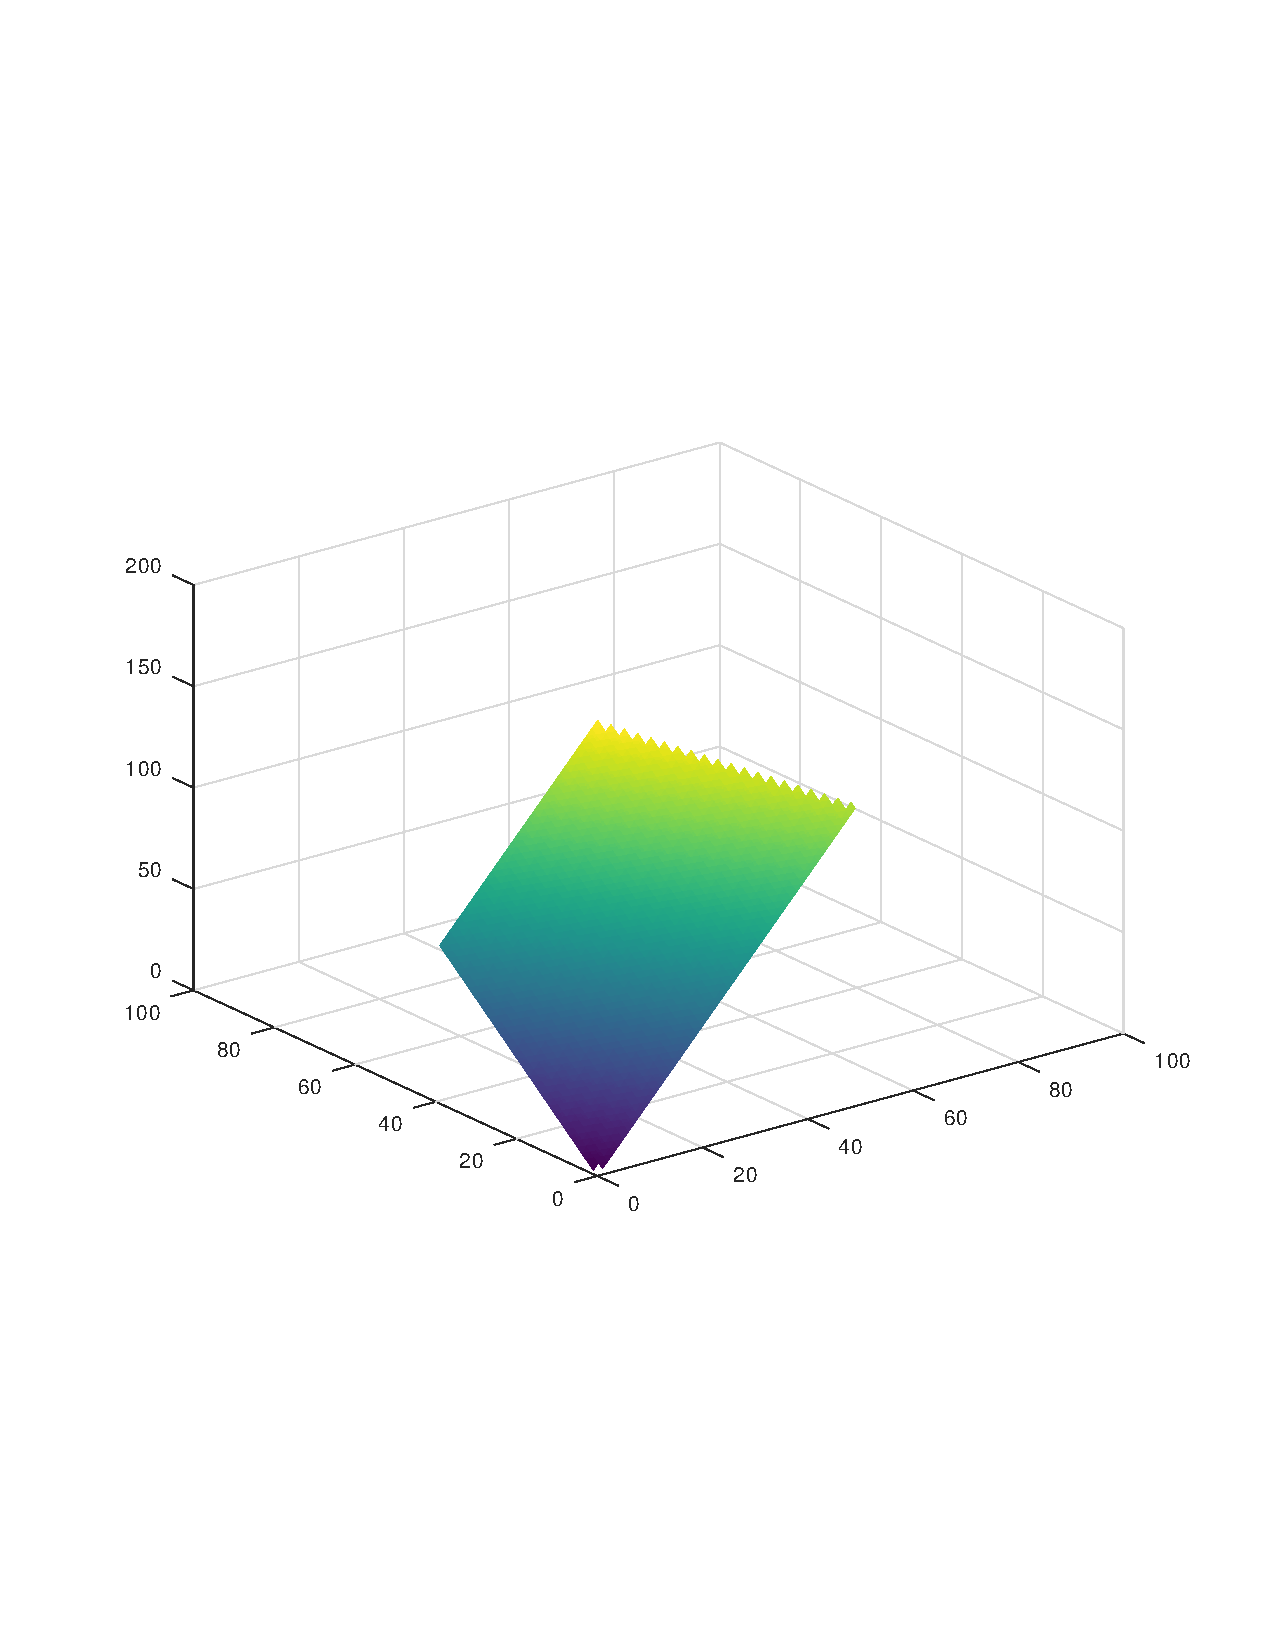
\includegraphics[width=\textwidth]{2_INTRO_3}
      \caption{La aplicación lineal $f$ restringida a $\mathcal{R}$}
    \end{subfigure}
  \end{figure}
}{
  \begin{figure}
    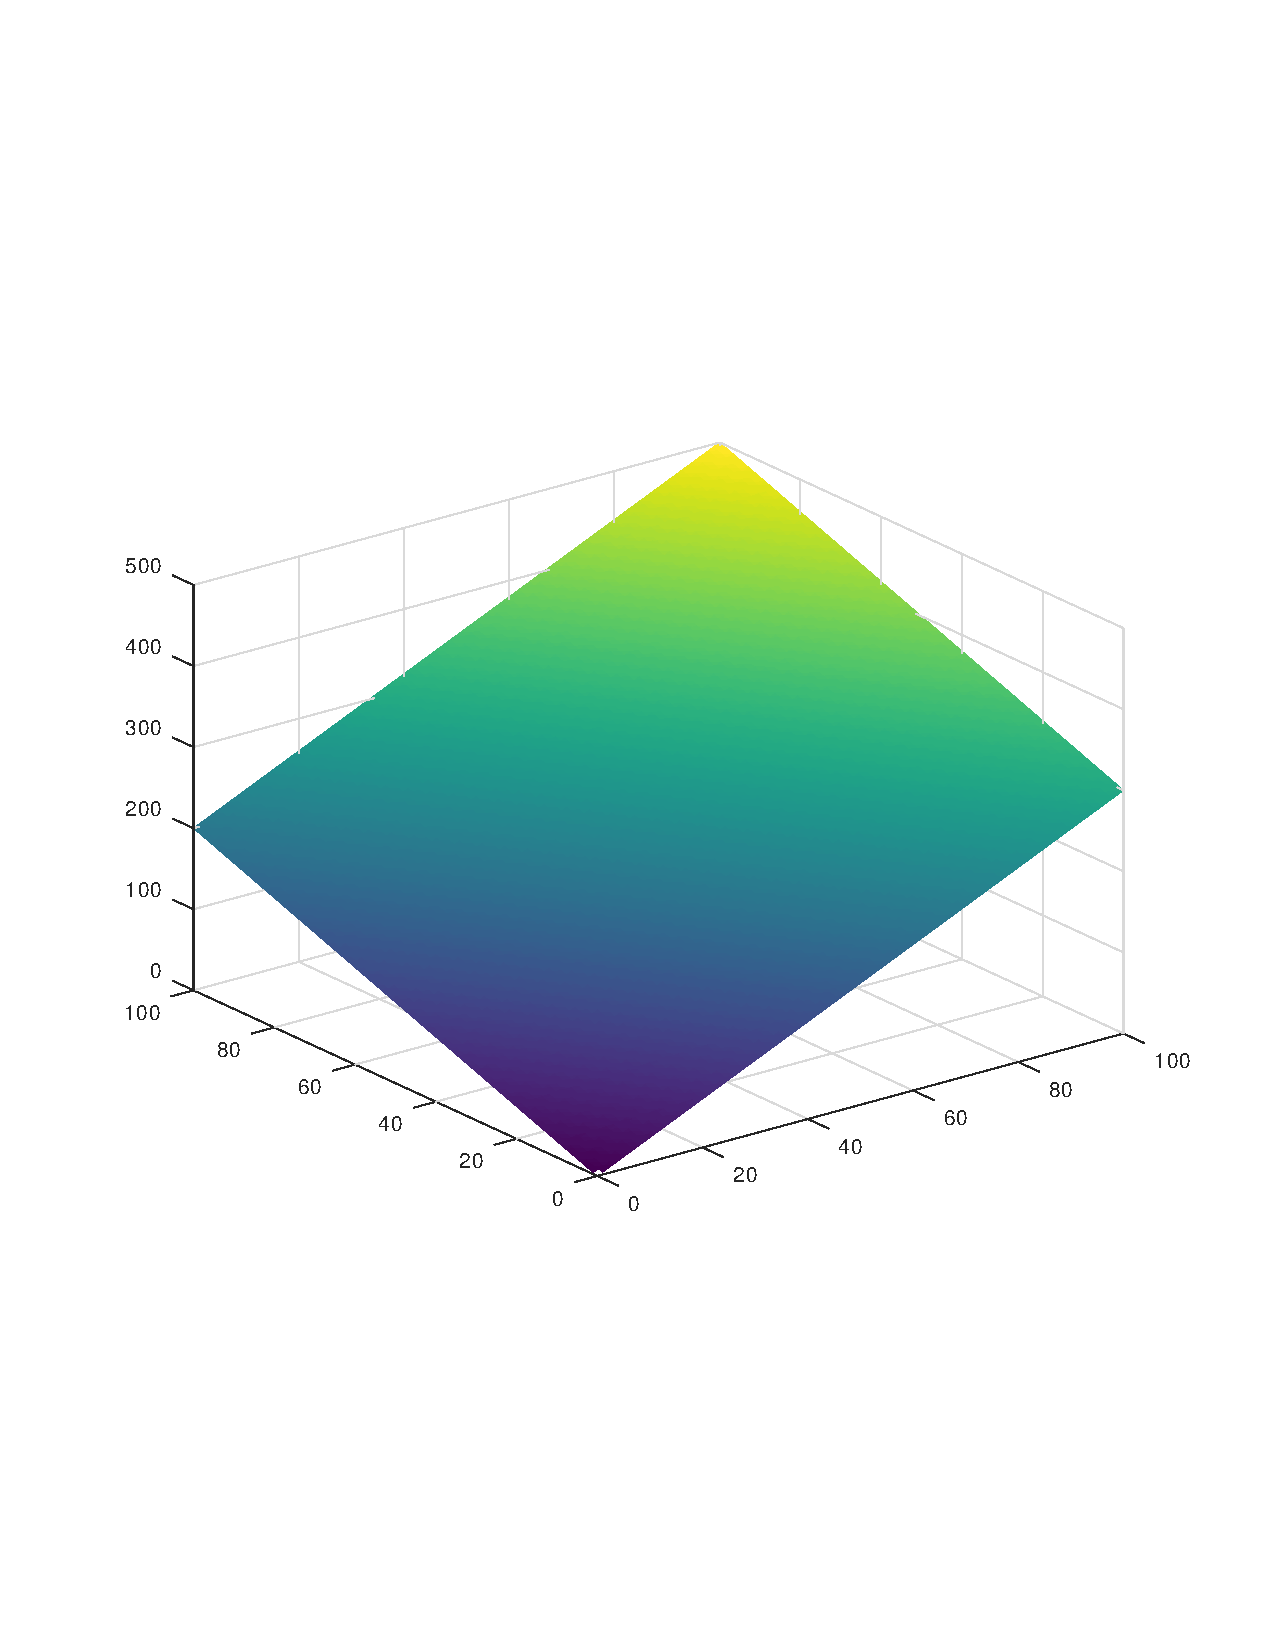
\includegraphics[width=\textwidth]{2_INTRO_1.pdf}
    \caption{Una aplicación $f$ lineal}
  \end{figure}

  \begin{figure}
    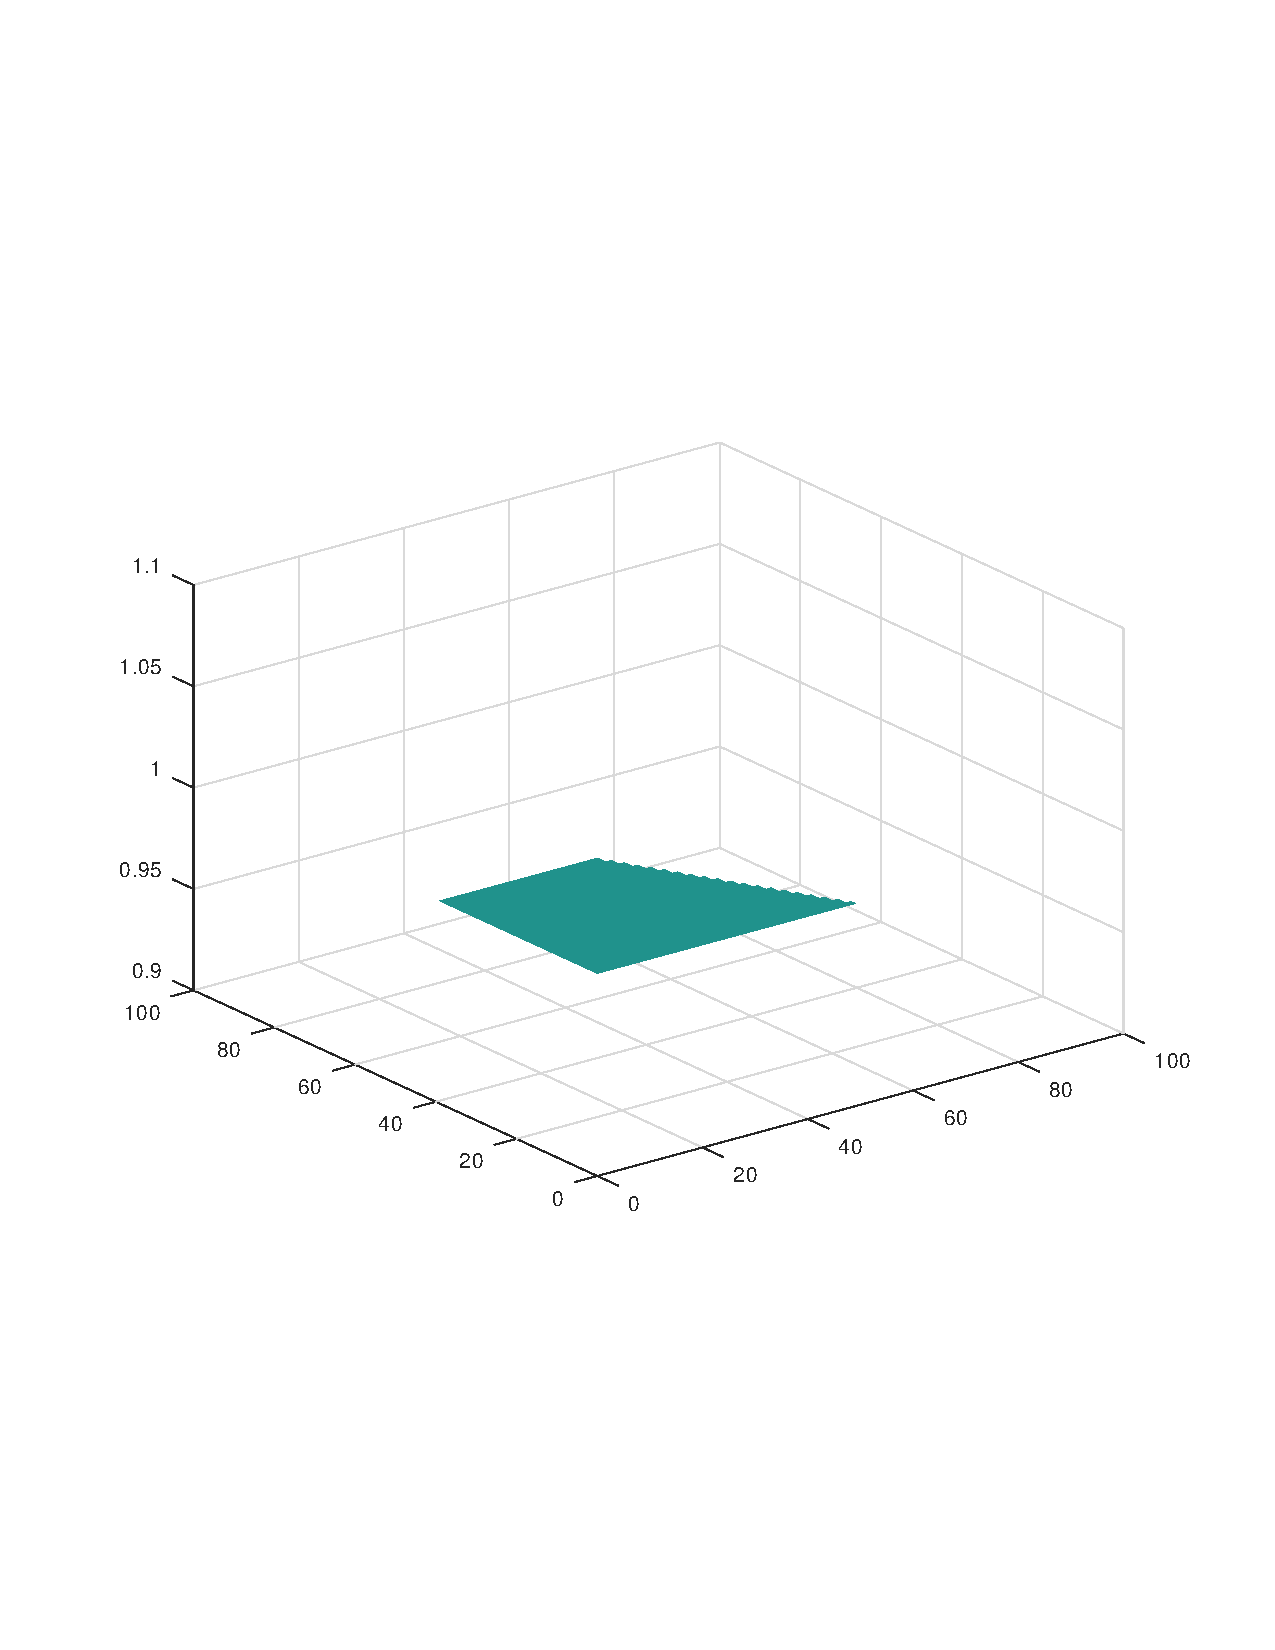
\includegraphics[width=\textwidth]{2_INTRO_2.pdf}
    \caption{Una $D$ región dada por restricciones}
  \end{figure}

  \begin{figure}
    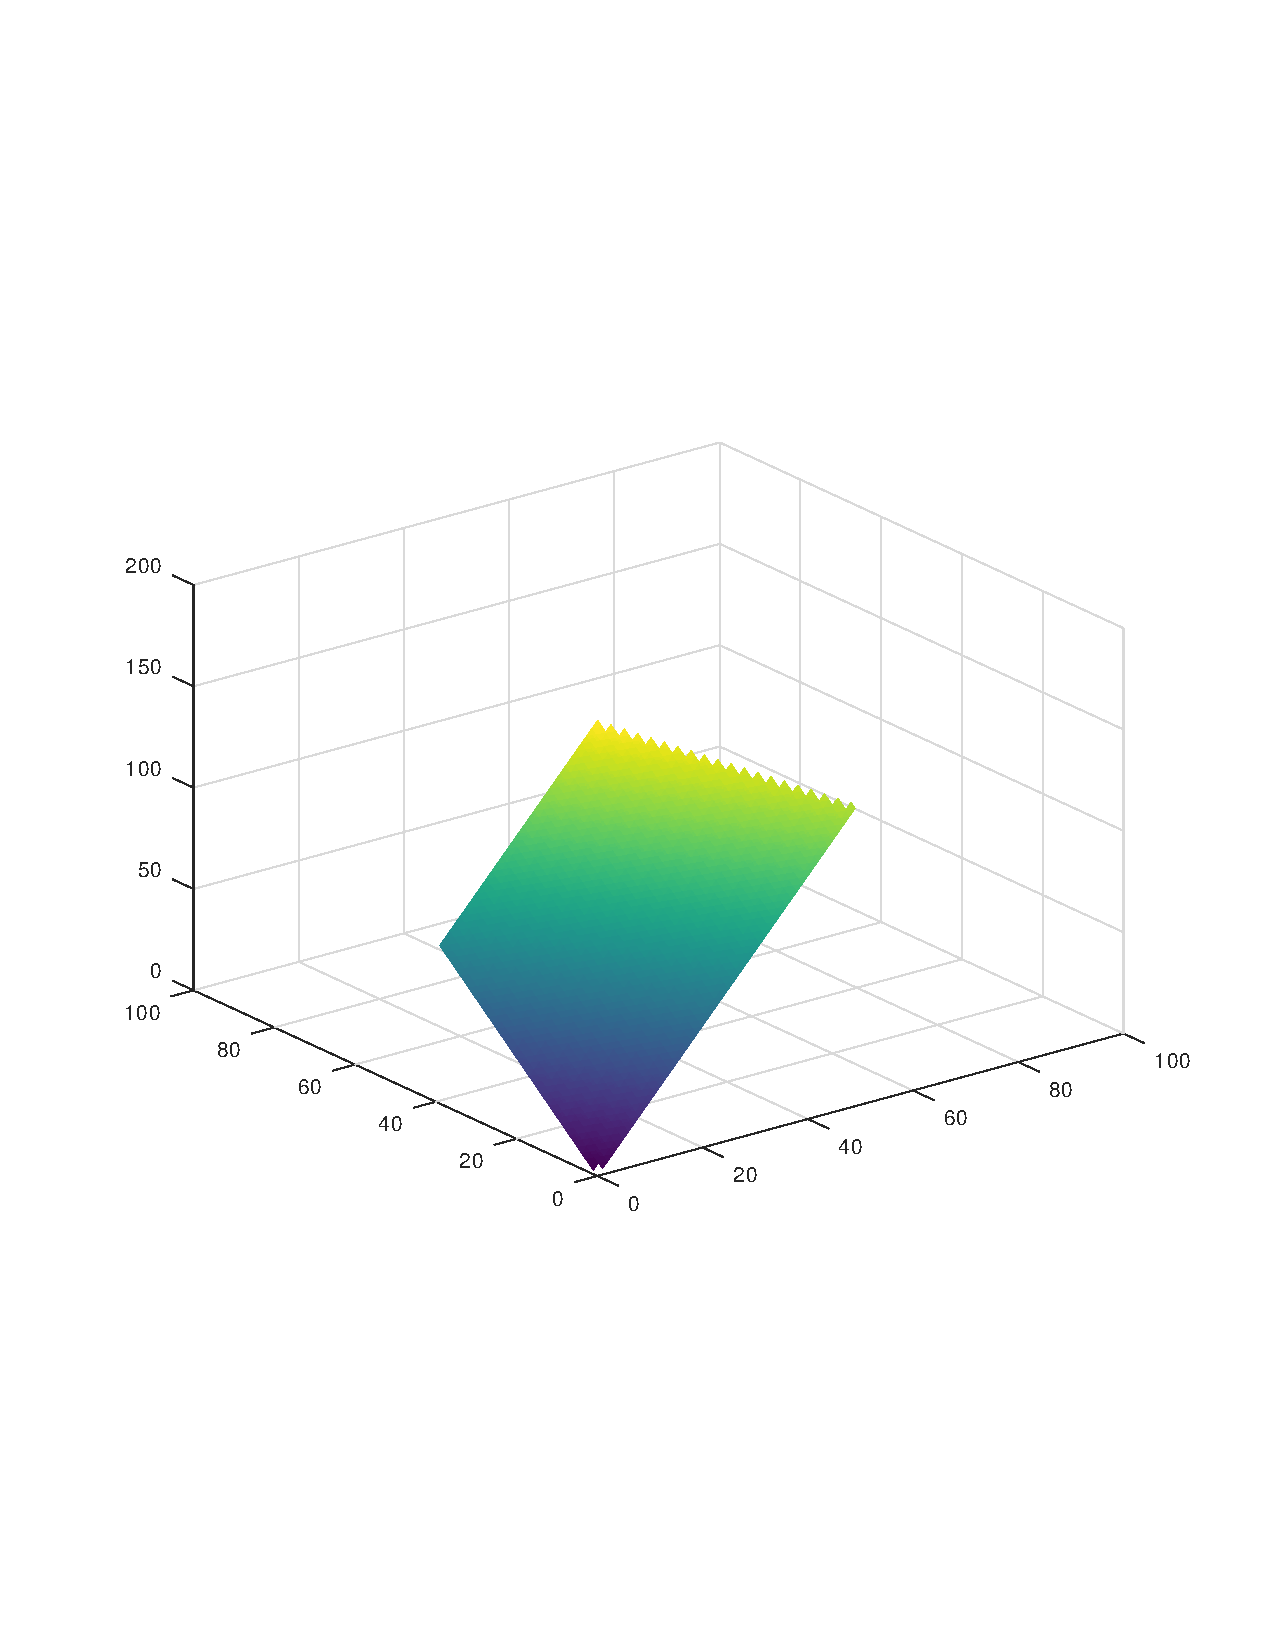
\includegraphics[width=\textwidth]{2_INTRO_3.pdf}
    \caption{La aplicación lineal $f$ restringida a $D$}
  \end{figure}
}
A la función $f:\IR^n\longrightarrow\IR$ se le pide que sea lineal y a $D$ que sea un conjunto definido por desigualdades lineales.